\documentclass{beamer}
\usepackage[utf8]{inputenc}
\usepackage{polski}
\usepackage[polish]{babel}
\usepackage{graphicx}
\usetheme{Darmstadt}

\newcommand{\impl}{\rightarrow}
\renewcommand{\implies}{\rightarrow}
\newcommand{\U}{\mathcal{U}}
\newcommand{\refl}[1]{\text{refl}_{#1}}

\title{Homotopiczna teoria typów}

\author{Zeimer}
\date{13 stycznia 2019}

\begin{document}

\frame{\titlepage}

\frame{\tableofcontents}

\section{Wstęp}

\begin{frame}{Czym jest HoTT?}
\begin{itemize}
	\item Homotopiczna teoria typów (w skrócie HoTT) to połączenie teorii typów i teorii homotopii.
	\item Jest kolejnym stadium ewolucji teorii typów.
	\item Jest syntetyczną teorią homotopii, dającą nam łatwy dostęp do skomplikowanych pojęć topologicznych.
	\item Jest pomysłem na nowe podstawy matematyki, alternatywne wobec teorii zbiorów.
	\item Jest bardzo potężnym funkcyjnym językiem programowania.
\end{itemize}
\end{frame}

\begin{frame}{Innowacje HoTT}
\begin{itemize}
	\item Homotopiczna interpretacja teorii typów, mocno wspomagająca wyobraźnię zarówno w rozumowaniu, jak i pozwalająca dogłębnie zrozumieć różne detale teorii typów.
	\item Aksjomat uniwalencji $(A \simeq B) \simeq (A = B)$, który głosi, że rzeczy mające tę samą strukturę są identyczne. Rozwiązuje to odwieczny problem nieformalnego utożsamiania poprzez nadużycie języka.
	\item Wyższe typy induktywne, pozwalające w teorii typów:
	\begin{itemize}
		\item Zdefiniować wiele niemożliwych dotychczas obiektów, np. typy ilorazowe albo prezentacje obiektów algebraicznych.
		\item Konstruktywnie rozwiązać wiele problemów, które dotychczas wymagały logiki klasycznej (konstrukcja liczb rzeczywistych Cauchy'ego)
		\item Wyrazić klasyczne pojęcia logiczne (dysjunkcja, kwantyfikator egzystencjalny, aksjomat wyboru) z niemożliwą wcześniej w teorii typów precyzją.
	\end{itemize}
\end{itemize}
\end{frame}

\section{Teoria homotopii}

\begin{frame}{Teoria homotopii 1 - homotopia}
\begin{itemize}
	\item Co to jest homotopia?
	\item Zgodnie z wikipedią, jeżeli $f$ i $g$ są funkcjami ciągłymi z przestrzeni topologicznej $X$ w przestrzeń topologiczną $Y$, to $H: X \times [0; 1] \to Y$ jest homotopią, gdy jest funkcją ciągłą spełniającą $H(0, x) = f(x) \land H(1, x) = g(x)$.
	\item Jeżeli nieco pogmeramy w symbolach, to możemy to zapisać tak: $H: [0; 1] \to (X \to Y)$ jest homotopią, gdy jest ciągła i spełnia $H(0) = f \land H(1) = g$.
	\item Nie przejmuj się, jeżeli definicja cię nie oświeca. Moim zdaniem władowanie jej do nazwy całej teorii jest głupie.
\end{itemize}
\end{frame}

\begin{frame}{Teoria homotopii 2 - ścieżka}
\begin{itemize}
	\item Bardziej podstawowym pojęciem jest ścieżka.
	\item Ścieżka w przestrzeni topologicznej $X$ to funkcja ciągła z $[0; 1]$ w $X$.
	\item Łatwo to sobie wyobrazić: odcinek $[0; 1]$ z pewnością jest ścieżką prowadzącą od $0$ do $1$. Jego obrazem, czyli ścieżką, jest więc pewien ciąły zawijasek, który prowadzi z $f(0)$ do $f(1)$.
	\item Ostatecznie możemy powiedzieć, że homotopia to ścieżka między funkcjami.
	\item Teoria homotopii nie jest jednak teorią ścieżek między funkcjami. Jest to raczej po prostu teoria ścieżek.
\end{itemize}
\end{frame}

\begin{frame}{Teoria homotopii 3 - topologia (algebraiczna)}
\begin{itemize}
	\item Po co to wszystko?
	\item Topologia jest całkiem użyteczna. Ostatnio popularna robi się topologiczna analiza danych. Zamiast prymitywnie przypasowywać do danych proste (regresja liniowa), ludzie próbują lepiej opisywać kształt danych. Topologia bada kształty, więc pasuje jak ulał.
	\item Chcemy więc wiedzieć więcej o topologii, np. czy dwie przestrzenie są takie same czy inne. Tutaj wkracza topologia algebraiczna, czyli dziedzina badająca przestrzenie topologiczne za pomocą metod algebraicznych.
\end{itemize}
\end{frame}

\begin{frame}{Teoria homotopii 4 - grupa podstawowa}
\begin{itemize}
	\item Pętla w punkcie $x$ to ścieżka, która zaczyna się i kończy w punkcie $x$.
	\item Grupa podstawowa przestrzeni $X$ w punkcie $x$ to grupa, której nośnikiem jest zbiór wszystkich pętli w punkcie $x$. Działaniem grupowym jest sklejanie pętli (najpierw pójdź pierwszą pętlą, a potem drugą). Odwrotność to pójście pętlą w przeciwnym kierunku. Element neutralny to stanie w miejscu.
	\item Grupa podstawowa jest fajna, bo jeżeli przestrzenie są izomorficzne, to ich grupy podstawowe też są. Wobec tego jeżeli grupy podstawowe (w dowolnym punkcie) są różne, to przestrzenie też są różne.
\end{itemize}
\end{frame}

\begin{frame}{Teoria homotopii 5 - okrąg i liczby całkowite}
\begin{itemize}
	\item Okrąg to taka przestrzeń topologiczna, że... wyobraź sobie, pewnie kiedyś widziałeś okrąg.
	\item Grupa podstawowa okręgu w dowolnym punkcie jest izomorficzna z grupą liczb całkowitych z dodawaniem.
	\item Stanie w miejscu reprezentuje $0$.
	\item $n$ okrążeń zgodnie z ruchem wskazówek zegara reprezentuje liczbę $n$.
	\item $n$ okrążeń przeciwnie do ruchu wskazówek zegara reprezentuje liczbę $-n$.
\end{itemize}
\end{frame}

\section{Teoria typów}

\begin{frame}{Teoria typów 1 - podstawy}
\begin{itemize}
	\item Teorię typów w ujęciu HoTTowym można opisać jako system formalny, który za pomocą reguł (osądów) opisuje byty zwane typami. Kluczową innowacją HoTT jest interpretacja typów i wymyślone na jej podstawie aksjomaty rzucające światło na naturę kosmosu.
	\item Reguły dzielą się na ciekawe i nieciekawe.
	\item Nieciekawe to te, które muszą być, żeby wszystko działało, np. do zamieniania kolejności rzeczy w kontekście.
	\item Ciekawe to te, które faktycznie opisują typy. Jest ich pięć rodzajów: reguły formacji, wprowadzania, eliminacji, obliczania i unikalności.
\end{itemize}
\end{frame}

\begin{frame}{Teoria typów 2 - pięć rodzajów reguł}
\begin{itemize}
	\item Reguły formacji mówią, skąd się biorą typy.
	\item Reguły wprowadzania mówią, jak zrobić elementy danego typu.
	\item Reguły eliminacji mówią, jak zrobić coś z elementami danego typu.
	\item Reguły obliczania mówią, jak reguły eliminacji mają się do reguł wprowadzania.
	\item Reguły unikalności mówią, jak reguły wprowadzania mają się do reguł eliminacji.
\end{itemize}
\end{frame}

\begin{frame}{Teoria typów 3 - reguły dla funkcji}

\begin{itemize}
	\item Ćwiczenie: nazwij każdą z reguł (tzn. która to reguła formacji, która obliczania etc.)
\end{itemize}

	\begin{center}
		$\displaystyle \frac{\Gamma \vdash A : \U \quad \Gamma \vdash B : \U}{\Gamma \vdash A \to B : \U}$
	\end{center}
	\begin{center}
		$\displaystyle \frac{\Gamma, x : A \vdash b : B}{\Gamma \vdash \lambda x:A.b : A \to B}$
	\end{center}
	\begin{center}
		$\displaystyle \frac{\Gamma \vdash f : A \to B \quad \Gamma \vdash x : A}{\Gamma \vdash f\ x : B}$
	\end{center}
	\begin{center}
		$\displaystyle \frac{\Gamma, x : A \vdash b : B \quad \Gamma \vdash a : A}{\Gamma \vdash (\lambda x:A.b)\ a \equiv b[x := a] : B}$
	\end{center}
	\begin{center}
		$\displaystyle \frac{\Gamma \vdash f : A \to B}{\Gamma \vdash \lambda x:A.f\ x \equiv f : A \to B}$
	\end{center}
\end{frame}

\begin{frame}{Teoria typów 4 - ciekawostki o regułach}
\begin{itemize}
	\item Każdy typ musi mieć regułę formacji - inaczej nie byłby typem.
	\item Jednak nie każdy typ musi mieć pozostałe reguły.
	\item Typ $\mathbf{0}$ nie ma reguły wprowadzania, bo jest pusty i nie ma żadnych elementów.
	\item Uniwersum nie ma reguły eliminacji.
	\item Typ $\mathbf{0}$ nie ma także reguły obliczania, co jest oczywiste - nie może jej mieć, skoro nie ma reguły wprowadzania.
	\item Wiele typów, np. sumy i produkty, nie mają reguły unikalności. W zamian za to mają one zdaniową regułę unikalności, tzn. można udowodnić twierdzenie wyglądające dokładnie jak reguła unikalności.
	\item Reguła formacji zawsze jest jedna, bo każdy typ można sformować tylko na jeden sposób. Pozostałych reguł może być więcej. Sumy mają 2 reguły wprowadzania, a produkty 2 reguły eliminacji i wobec tego 2 reguły obliczania.
\end{itemize}
\end{frame}

\begin{frame}{Teoria typów 5 - trzy style definiowania}
\begin{itemize}
	\item Formalnie rzeczy definiujemy za pomocą reguł wprowadzania i eliminacji.
	\item Przykład: funkcję $\text{swap} : \Pi A\ B : \U. A \times B \to B \times A$ możemy zdefiniować jako $\text{swap} :\equiv \lambda A : \U.\lambda B : \U.\lambda x : A \times B. (\pi_2\ x, \pi_1\ x)$
	\item Zamiast tego często będziemy jednak definiować poprzez dopasowanie do wzorca, jednocześnie pomijając argumenty, które można wywnioskować z kontekstu: $\text{swap}\ (a, b) :\equiv (b, a)$
	\item Możemy też definiować słownie: niech $\text{swap}$ będzie funkcją, która zamienia miejscami elementy pary. Ten sposób będziemy wykorzystywać do dowodzenia twierdzeń.
\end{itemize}
\end{frame}

\section{Interpretacja homotopiczna}

\begin{frame}{Interpretacja typów 1 - zbiory}
\begin{itemize}
	\item Jak interpretować/rozumieć typy?
	\item Najprostszy sposób każe nam myśleć, że typy to po prostu zbiory.
	\item W takim ujęciu typ $\mathbb{N}$ to taki worek, w którym jest $0, 1, 2, \dots$ etc.
	\item Takie rozumienie było przez długi czas dominujące. Jest ono dość intuicyjne i powszechne przy myśleniu nieformalnym.
	\item Były też inne dziwne interpretacje, jak (chyba) częściowe relacje równoważności, ale kogo to obchodzi.
\end{itemize}
\end{frame}

\begin{frame}{Interpretacja typów 2 - grupoidy}
\begin{itemize}
	\item Aż tu nagle w pracy z 1995 zatytułowanej ``The groupoid interpretation of type theory'' panowie Hofmann i Streicher wpadli na pomysł, żeby zinterpretować typy jako grupoidy.
	\item Upraszczając, grupoid to graf skierowany, w którym:
	\begin{itemize}
		\item Każdy wierzhołek ma krawędź do samego siebie.
		\item Jeżeli jest krawędź z $A$ do $B$, to jest krawędź z $B$ do $A$.
		\item Jeżeli jest krawędź z $A$ do $B$ i z $B$ do $C$, to jest krawędź z $A$ do $C$.
	\end{itemize}
	\item Jeszcze bardziej upraszczając: grupoid to kolekcja kropek, między którymi są strzałki spełniające pewne warunki.
	\item Wymyślenie ciągu dalszego tej bajki zajęło dobre 15 lat.
\end{itemize}
\end{frame}

\begin{frame}{Interpretacja typów 3 - $\omega$-grupoidy}
\begin{itemize}
	\item Aż tu nagle w okolicach roku 2010 Awodey i Warren (a także Voevodsky, van den Berg i Garner) wpadli na pomysł, żeby zinterpretować typy jako $\omega$-grupoidy.
	\item $\omega$-grupoid to kolekcja kropek, między którymi są strzałki spełniające warunki jak dla grupoidu. Co więcej, między strzałkami też mogą być strzałki spełniające te warunki. Są też strzałki między strzałkami między strzałkami i tak dalej aż do nieskończoności.
	\item Jeżeli pomyślimy o naszych ``strzałkach'' jak o ścieżkach w przestrzeni, to dostajemy homotopiczną interpretację teorii typów. W zasadzie to każdy $\omega$-grupoid jest reprezentacją jakiejś przestrzeni topologicznej.
\end{itemize}
\end{frame}

\begin{frame}{1.12 Ścieżki 1 - reguły}
\makebox[\linewidth]{\parbox{12cm}
{
	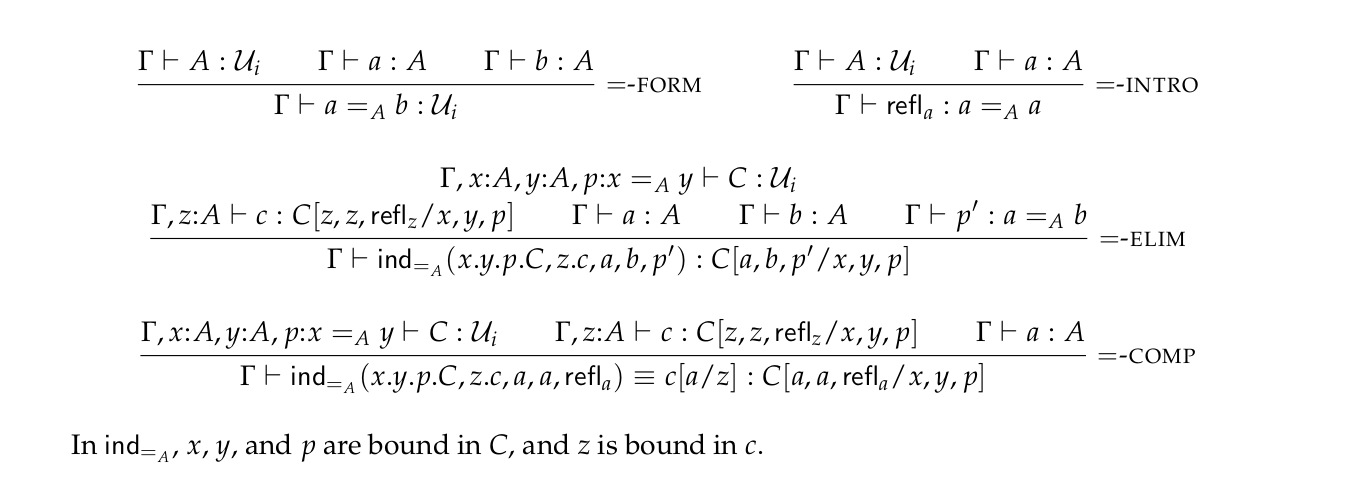
\includegraphics[scale=0.25]{IdentityTypesSmall.png}}
}
Powyższe reguły opisują rodzinę typów, która zazwyczaj nazywana bywa typem identycznościowym (ang. identity type), ale zgodnie z interpretacją homotopiczną będę go nazywał typem ścieżek.
\end{frame}

\begin{frame}{1.12 Ścieżki 2 - interpretacja reguł}
\begin{itemize}
	\item Reguła formacji: jeżeli mamy typ $A$ i dwa jego elementy $a, b$, to możemy sformować typ $a =_A b$. Jest to typ, którego elementami są ścieżki z $a$ do $b$. Jeżeli mamy element tego typu, to $a$ i $b$ są równe.
	\item Reguła wprowadzania: każda rzecz jest równa sama sobie. Ścieżka poświadczająca ten fakt nazywa się $\text{refl}$. Jest to skrót od ang. reflexivity, czyli zwrotność.
	\item Reguła eliminacji: $C$ jest tutaj rodziną typów zależącą od ścieżki $p : x = y$. Reguła głosi, że żeby zdefiniować element $C(x, y, p)$ wystarczy mieć element $C(x, x, \refl{x})$.
	\item Reguła obliczania: chodzi o to, że jeżeli wyeliminujemy element $C(z, z, \refl{z})$, to dostaniemy go spowrotem, tylko po odpowiednim podstawieniu.
\end{itemize}
\end{frame}

\begin{frame}{1.12 Ścieżki 3 - indukcja po ścieżkach}
\begin{itemize}
	\item Reguła eliminacji dla ścieżek nosi nazwę indukcji po ścieżkach (ang. path induction).
	\item Zaprezentowany powyżej wariant precyzyjniej nazywa się unbased path induction. Polega na zastąpieniu dwóch obiektów $a, b$ i ścieżki $p$ przez generyczny obiekt $z$ i ścieżkę $\refl{z}$.
	\item Inny wariant nosi nazwę based path induction. Polega on na zastąpieniu obiektu $b$ przez obiekt $a$ oraz ścieżki $p : a = b$ przez ścieżkę $\refl{a}$.
	\item Oba warianty są równoważne. Dowód: HoTT Book, podrozdział 1.12.2.
\end{itemize}
\end{frame}

\begin{frame}{1.12 Ścieżki 4 - interpretacja indukcji po ścieżkach}
\begin{itemize}
	\item Tak jak indukcję na liczbach naturalnych możemy zobrazować za pomocą domina, tak indukcję po ścieżkach możemy wyobrażać sobie jako ściągnięcie/zwinięcie ścieżki $p : a = b$ do ścieżki trywialnej.
	\item W wariancie unbased oba końce ścieżki $p$ są wolne. Wybieramy jakiś punkt $z$ na ścieżce i ciągniemy oba końce w jego kierunku. Ostatecznie dostajemy ścieżkę $\refl{z}$.
	\item W wariancie based lewy koniec ścieżki $p$ jest sztywny, a prawy jest wolny. Chwytamy więc prawy koniec $b$ i ciągniemy go po ścieżce w kierunku lewego końca $a$. Ostatecznie dostajemy ścieżkę $\refl{a}$.
	\item Zauważmy, że jeżeli oba końce ścieżki są sztywne, to nie możemy robić indukcji - spróbuj pociągnąć linę okręconą wokół latarni. O tym, czy koniec jest sztywny czy wolny, decyduje to, czy jest skwantyfikowany uniwersalnie czy nie.
\end{itemize}
\end{frame}

\begin{frame}{1.12 Ścieżki 5 - wątpliwości i ciekawostki}
\begin{itemize}
	\item Reguła eliminacji dla typu $\text{bool}$ intuicyjnie mówi, że jedynymi elementami typu $\text{bool}$ są $\text{true}$ oraz $\text{false}$.
	\item Czy więc indukcja po ścieżkach mówi, że jedyną ścieżką jest $\text{refl}$?
	\item Zanim odpowiemy, garść ciekawostek.
	\item Indukcja po ścieżkach nie jest HoTTową innowacją. Jedynie nazwa jest nowa. W teorii typów bywa często nazywana $J$.
	\item Zdanie mówiące, że każda ścieżka jest trywialna, nazywa się ``Aksjomat $K$''.
	\item Związek z facetami w czerni jest przypadkowy.
	\item Inne zdanie, mówiące że jest tylko jedna ścieżka, nazywa się w ang. UIP, co jest skrótem od ``Uniqueness of Identity Proofs''.
	\item To właśnie badanie nad tego typu zagadnieniami doprowadziły do homotopicznej interpretacji teorii typów.
\end{itemize}
\end{frame}

\begin{frame}{1.12 Ścieżki 6 - rozwianie wątpliwości}
\begin{itemize}
	\item Indukcja po ścieżkach nie głosi, że jest tylko jedna ścieżka.
	\item Formalna różnica jest taka, że typ $\text{bool}$ jest generowany induktywnie, podczas gdy w przypadku ścieżek, które są rodziną typów, to cała rodzina jest generowana induktywnie, a nie pojedynczy typ $x = y$.
	\item Parafrazując, nie można w tym przypadku rozważać samych ścieżek w oderwaniu od ich końców.
	\item Nie możemy zatem udowodnić, że każda ścieżka $p : x = x$ jest trywialna.
	\item Ale możemy udowodnić, że każda ścieżka razem z jej końcami jest trywialna: zachodzi $(x, y, p) = (x, x, \refl{x})$, gdzie równość jest w typie $\Sigma x\ y : A, x = y$. Odpowiada to indukcji po ścieżkach w wersji unbased.
	\item Podobnie dla ustalonego $a : A$ możemy pokazać, że $(x, p) = (a, \refl{a})$ w typie $\Sigma x : A, a = x$. Odpowiada to indukcji po ścieżkach w wersji based.
\end{itemize}
\end{frame}

\begin{frame}{2.1 Typy to wyższe grupoidy}
\begin{itemize}
	\item todo
\end{itemize}
\end{frame}

\begin{frame}{2.2 Funkcje to funktory}
\begin{itemize}
	\item todo
\end{itemize}
\end{frame}

\begin{frame}{2.3 Mu synku mu, czyli transport}
\begin{itemize}
	\item todo
\end{itemize}
\end{frame}

\begin{frame}{2.4 Homotopie i równoważności}
\begin{itemize}
	\item todo
\end{itemize}
\end{frame}

\begin{frame}{2.5-2.8 Wyższogrupoidowa struktura typów}
\begin{itemize}
	\item todo
\end{itemize}
\end{frame}

\begin{frame}{2.9 Ekstensjonalność}
\begin{itemize}
	\item todo
\end{itemize}
\end{frame}

\begin{frame}{2.10 Uniwalencja}
\begin{itemize}
	\item todo
\end{itemize}
\end{frame}

\begin{frame}{Innowacje HoTT w przykładach - uniwalencja 1}
\begin{itemize}
	\item Rozważmy dwa poniższe typy (tak naprawdę powinniśmy też podać reguły eliminacji i obliczania, ale nie są one istotne dla przykładu).
	\item Niech $\mathbb{N} :\equiv 0 \: | \: S\ \mathbb{N}$ i niech $\mathbb{N}' :\equiv 0' \: | \: S'\ \mathbb{N}'$
	\item Rodzi się pytanie: czy $\mathbb{N}$ i $\mathbb{N}'$ to to samo, czy coś innego?
	\item Odpowiedź klasyczna: istnieje oczywisty izomorfizm $\mathbb{N} \cong \mathbb{N}'$. Na mocy nadużycia języka będziemy utożsamiać $\mathbb{N}$ i $\mathbb{N}'$, tzn. traktować je tak, jakby $\mathbb{N} = \mathbb{N}'$ mimo, że formalnie tak nie jest.
	\item Odpowiedź HoTTowa: istnieje oczywista równoważność $e : \mathbb{N} \simeq \mathbb{N}'$. Wobec tego na mocy aksjomatu uniwalencji mamy ścieżkę $\text{ua}(e) : \mathbb{N} = \mathbb{N}'$.
\end{itemize}
\end{frame}

\begin{frame}{Innowacje HoTT w przykładach - uniwalencja 2}
\begin{itemize}
	\item Aksjomat uniwalencji nie tylko usuwa nieprzyjemny filozoficzny smrodek, ale daje nam też nowe sposoby rozumowania.
	\item Przykład: każda równoważność jest monomorfizmem.
	\item Dowód klasyczny: każda równoważność ma odwrotność. Użyj jej.
	\item Dowód HoTTowy: każda równoważność pochodzi od jakiejś ścieżki. Na mocy indukcji po ścieżkach możemy założyć, że ścieżka ta jest trywialna, a zatem nasza równoważność jest identycznością.
\end{itemize}
\end{frame}

\begin{frame}{2.14 Przykład: równość struktur}
\begin{itemize}
	\item todo
\end{itemize}
\end{frame}

\section{Zbiory i logika}

\begin{frame}{Hierarchia n-typów}
\begin{itemize}
	\item Hierarchia n-typów: unit, funkcje sortujące, pusty, zbiory, grupoidy, okrąg, uniwersum.
	
\end{itemize}
\end{frame}

\begin{frame}{Metoda encode-decode dla liczb naturalnych}
\begin{itemize}
	\item todo - przenieść to w miejsce, gdzie już wiadomo, co to zbiory
\end{itemize}
\end{frame}

\begin{frame}{3.11 Kontraktowalność}
\begin{itemize}
	\item todo
\end{itemize}
\end{frame}

\begin{frame}{3.3 Zdania}
\begin{itemize}
	\item todo
\end{itemize}
\end{frame}

\begin{frame}{3.1 Zbiory}
\begin{itemize}
	\item todo
\end{itemize}
\end{frame}

\begin{frame}{3.7 Trunkacja}
\begin{itemize}
	\item todo
\end{itemize}
\end{frame}

\begin{frame}{3.4 Logika klasyczna i intuicjonistyczna}
\begin{itemize}
	\item todo
\end{itemize}
\end{frame}

\begin{frame}{Innowacje HoTT w przykładach - logika 1}
\begin{itemize}
	\item Znaczenie klasycznej dysjunkcji jest inne, niż konstruktywnej. Klasycznie $P \lor Q$ znaczy, że zachodzi $P$ lub $Q$ lub oba na raz, ale nie wiemy, które. Konstruktywnie $P \lor Q$ znaczy, że zachodzi $P$ lub $Q$ i wiemy, z którym przypadkiem mamy do czynienia
\end{itemize}
\end{frame}

\begin{frame}{3.8 Aksjomat Wyboru}
\begin{itemize}
	\item
\end{itemize}
\end{frame}

\begin{frame}{Innowacje HoTT w przykładach - logika 2}
\begin{theorem}[Aksjomat wyboru]
$\textstyle \prod (A : \mathcal{U}) (B : A \to \mathcal{U}) (R : \Pi x : A, B\ x \to \mathcal{U}),$ \\
	$\textstyle \quad (\prod x : A, \sum y : B\ x, R\ x\ y) \to$ \\
		$\textstyle \qquad \sum f : (\Pi x : A, B\ x), \Pi x : A, R\ x\ (f\ x)$
\end{theorem}
\begin{proof}
	Na tablicy.
\end{proof}

Powyższe twierdzenie jest problematyczne, gdyż wygląda jak aksjomat wyboru, ale nie ma tutaj żadnego wybierania.

\end{frame}

\begin{frame}{3.9 Zasada unikalnego wyboru}
\begin{itemize}
	\item
\end{itemize}
\end{frame}

\begin{frame}{wut}
\begin{itemize}
	\item
\end{itemize}
\end{frame}

\section{Równoważności}

\begin{frame}{4.2-4.5 Różne oblicza równoważności}
\begin{itemize}
	\item
\end{itemize}
\end{frame}

\begin{frame}{4.6 Surjekcje i injekcje}
\begin{itemize}
	\item
\end{itemize}
\end{frame}

\begin{frame}{Wielkie odkrycie filozoficzne - injekcja to surjekcja}
\begin{itemize}
	\item
\end{itemize}
\end{frame}

\begin{frame}{Bibliografia}
\begin{itemize}
	\item Podstawowym źródłem wiedzy jest książka \url{https://homotopytypetheory.org/book/}
	\item Jakaś prezentacja: \url{http://www.cs.nott.ac.uk/~psztxa/talks/edinburgh-13.pdf}
	\item Filozoficzne wynurzenia: \url{https://www.researchgate.net/publication/280671356_Does_Homotopy_Type_Theory_Provide_a_Foundation_for_Mathematics}
	\item Wesoły papiur o trunkacji i topologicznych rzeczach: \url{https://arxiv.org/pdf/1610.03346.pdf}
\end{itemize}
\end{frame}

\end{document}